\documentclass[11pt,a4paper]{article}

% ---- Packages ----
\usepackage[T1]{fontenc}
\usepackage[utf8]{inputenc}
\usepackage{mathptmx}           % Times font (De Gruyter standard serif)
\usepackage[margin=2.5cm]{geometry}
\usepackage{graphicx}
\usepackage{booktabs}
\usepackage{amsmath,amssymb}
\usepackage{xcolor}
\usepackage{hyperref}
\usepackage{cleveref}
\usepackage[authoryear,round]{natbib}  % Harvard-style author-date citations
\usepackage{caption}
\usepackage{subcaption}
\usepackage{multirow}
\usepackage{float}
\usepackage{url}
\usepackage{lineno}           % Line numbering for review

\hypersetup{
  colorlinks=true,
  linkcolor=blue!60!black,
  citecolor=blue!60!black,
  urlcolor=blue!60!black,
}

\captionsetup{font=small, labelfont=bf}

% Revision change-marking: new/modified passages are set in blue for the editor.
% \long so the argument may contain paragraph breaks and display equations.
\long\def\rev#1{{\color{blue!70!black}#1}}

% ---- Title ----
\title{%
  Latent Truth Without a Gold Standard:\\
  Multi-Reference Credibility Modeling and Claim Governance\\
  for Gene-Regulatory-Network Benchmarking%
}

\author{%
  Ihor Kendiukhov\textsuperscript{*}\\[4pt]
  {\normalsize Department of Computer Science, University of T\"ubingen, T\"ubingen, Germany}\\[2pt]
  {\normalsize \texttt{kenduhov.ig@gmail.com}}\\[2pt]
  {\small ORCID: \url{https://orcid.org/0000-0001-5342-1499}}
}

\date{}

\begin{document}
\linenumbers
\maketitle

\renewcommand{\thefootnote}{\fnsymbol{footnote}}
\footnotetext[1]{Corresponding author: Ihor Kendiukhov, Department of Computer Science, University of T\"ubingen, Sand 14, 72076 T\"ubingen, Germany. E-mail: kenduhov.ig@gmail.com}
\renewcommand{\thefootnote}{\arabic{footnote}}

% ======================================================================
% ABSTRACT
% ======================================================================
\begin{abstract}
Gene-regulatory-network (GRN) inference from single-cell foundation models is typically benchmarked against a single curated reference, even though available references are incomplete, noisy, and context-biased.
We propose a multi-reference latent truth framework that treats each reference database as a noisy evidence channel and estimates per-edge credibility under explicit source dependence.
We compare five latent-truth estimators of increasing complexity and find that a hierarchical family-Bayes model achieves the lowest rank disagreement under both source-dropout and family-block-dropout stress tests on a 421,521-edge candidate space.
A dual-universe evaluation contrasts a full candidate space with a context-matched universe.
\rev{The raw precision and F1 gap between the two contexts is large (23--31$\times$), but we show through an explicit decomposition that it is almost entirely a base-rate artifact: the context-matched universe has a $25.8\times$ higher density of evaluable perturbation references, so once metrics are normalized to a denominator-invariant enrichment-over-random the genuine ranking difference between contexts is modest ($\approx$1.4$\times$). This reconciles the apparent uplift with universe-aware evaluation and motivates reporting prevalence-normalized enrichment rather than raw precision.}
We introduce a four-tier dual-universe claim governance policy that restricts promotion to edges supported in both evaluation contexts and show that it reduces overpromotion to 0.2\% of the candidate space while achieving denominator-invariant perturbation-backed enrichment of $2.2\times$ ($p \ll 0.05$) on pre-registered panels.
\rev{The promoted set is further validated against a genuinely external ChIP-seq reference (ENCODE, never used in the fusion), where it is enriched $1.77\times$--$2.12\times$ ($p<10^{-7}$), with a clean monotone separation across governance tiers.}
Leave-one-cohort-out replication across six perturbation cohorts yields a pass rate of 5/6, with the single failure explained by sparse reference support ($<$10 edges); \rev{given the small number of cohorts, we treat this as an exploratory reliability threshold rather than a definitive operating boundary.}
All analyses run on laptop-scale table-level pipelines, requiring no GPU compute.
\end{abstract}

\noindent\textbf{Keywords:} gene regulatory networks; benchmarking; latent truth model; multi-reference fusion; mechanistic interpretability; single-cell foundation models

% ======================================================================
% 1. INTRODUCTION
% ======================================================================
\section{Introduction}\label{sec:intro}

Single-cell foundation models such as scGPT~\citep{cui2024scgpt} and Geneformer~\citep{theodoris2023transfer} have demonstrated the capacity to learn biologically meaningful representations of gene regulation from large-scale transcriptomic atlases.
A growing body of work has sought to extract gene-regulatory-network (GRN) predictions from model internals, including attention weights, gradient-based attributions, and probing classifiers~\citep{hao2024large}.
Evaluating the accuracy of these predicted networks, however, depends on comparison to curated reference databases such as TRRUST~\citep{han2018trrust} and DoRothEA~\citep{garcia2019benchmark}, which are themselves incomplete, noisy, and biased toward well-studied genes and pathways.

The standard practice of treating a single reference as ground truth introduces at least three problems.
First, different references can produce materially different method rankings for the same predictions, because each database captures a different slice of the true regulatory landscape~\citep{pratapa2020benchmarking}.
Second, reference completeness varies sharply by biological context: databases curated primarily from immune cells may not reflect regulatory logic in metabolic or developmental tissues~\citep{schiebinger2019optimal, kamimoto2023dissecting}.
Third, correlated curation biases across reference families (for example, databases that share upstream literature sources) can inflate apparent agreement without improving biological fidelity.

In this paper, we address these challenges by proposing a \emph{multi-reference latent truth framework} that replaces the single-reference assumption with an explicit probabilistic model of reference credibility.
The key idea is that each reference database is treated as a noisy observation of an unobserved latent truth about whether a regulatory edge is real, and credibility is estimated by modeling the dependence structure among sources.
We make four contributions:

\begin{enumerate}
  \item We develop a family of five latent-truth estimators of increasing sophistication, culminating in a hierarchical family-Bayes model that pools information across correlated reference families while preserving source-specific signal.
  \item We introduce a \emph{dual-universe evaluation} framework that measures perturbation calibration in both a full candidate space (421,521 edges) and a context-matched universe (7,536 edges). \rev{We show that the large apparent gap in raw precision between these contexts is driven overwhelmingly by their differing reference density (a denominator effect), and advocate reporting denominator-invariant enrichment-over-random as the universe-aware quantity of interest.}
  \item We propose a four-tier \emph{claim governance} policy that cross-references evidence from both universes and restricts edge promotion to those with consistent support, reducing overconfident claims from hundreds of thousands to 842 promotion-eligible edges. \rev{We provide exact tier definitions, a $\pm$10\% cutoff sensitivity analysis, a per-tier risk/return breakdown, an automated diversity--precision operating-point selector, and a functional characterization of the promoted set.}
  \item We validate the framework through pre-registered leave-one-cohort-out replication across six perturbation datasets \rev{and against a genuinely external ChIP-seq reference set (ENCODE) that is not used anywhere in the credibility model}, identifying an exploratory reliability threshold based on reference support density.
\end{enumerate}

All analyses run on laptop-scale table-level pipelines requiring no GPU compute, making the framework accessible for routine benchmarking workflows.

% ======================================================================
% 2. RELATED WORK
% ======================================================================
\section{Related Work}\label{sec:related}

\paragraph{GRN inference and benchmarking.}
Classical GRN inference methods, including GENIE3~\citep{huynh2010inferring}, GRNBoost2~\citep{moerman2019grnboost2}, and SCENIC~\citep{aibar2017scenic}, recover regulatory relationships from expression data using tree-based or correlation-based approaches.
Benchmarking studies have documented substantial protocol sensitivity, with method rankings changing depending on reference choice, preprocessing pipeline, and evaluation metric~\citep{pratapa2020benchmarking}.
Recent work has extended inference to single-cell foundation model internals, but the evaluation methodology has largely inherited single-reference assumptions from the classical setting.

\paragraph{Multi-source data fusion and latent truth models.}
The problem of estimating a latent truth from multiple noisy sources has a long history in statistics and machine learning.
The Dawid--Skene model~\citep{dawid1979maximum} and its extensions, including the Bayesian formulation of \citet{raykar2010learning}, model annotator reliability to infer true labels from noisy crowd-sourced annotations.
In genomics, meta-analytic approaches have been used to combine evidence across studies~\citep{tseng2012comprehensive}, but typically assume source independence and equal weighting rather than modeling explicit dependence structures.
Our work adapts the latent-truth paradigm specifically to GRN reference databases, incorporating family-level dependence to account for correlated curation biases.

\paragraph{Evaluation bias in GRN recovery.}
Several recent studies have highlighted how evaluation choices can bias GRN benchmarking conclusions.
Candidate-set composition, symbol-mapping conventions, and metric selection can each produce ranking reversals among methods that appear comparable~\citep{pratapa2020benchmarking, jackson2020gene}.
Context dependence of evaluation, where reference coverage varies across tissues and cell states, has been documented but not systematically addressed through multi-reference modeling~\citep{bravo2023scenic}.
\rev{A closely related diagnostic point is that restricting the candidate set to known regulator--target pairs inflates precision-type metrics by one to three orders of magnitude relative to a universe-aware evaluation over all biologically plausible pairs, purely through the change in denominator~\citep{kendiukhov2025universe}. The present work is the constructive counterpart to that diagnosis: rather than choosing a single candidate universe, we evaluate in two universes simultaneously, decompose the resulting metric gap into its denominator and signal components, and use denominator-invariant enrichment for all promotion decisions.}

\paragraph{Perturbation-grounded validation.}
CRISPR perturbation datasets, including Perturb-seq screens from \citet{dixit2016perturb}, \citet{adamson2016multiplexed}, and the Perturb-seq atlas of \citet{replogle2022mapping}, provide partial external anchors for GRN predictions.
However, perturbation coverage is sparse relative to the full space of predicted regulatory edges, and overlap with curated references varies by tissue context~\citep{kamimoto2023dissecting}.

% ======================================================================
% 3. METHODS
% ======================================================================
\section{Methods}\label{sec:methods}

\subsection{Problem Formulation}\label{sec:problem}

Let $\mathcal{E} = \{e_1, \ldots, e_N\}$ denote a set of $N$ candidate regulatory edges predicted from a foundation model, and let $\mathcal{S} = \{s_1, \ldots, s_K\}$ denote $K$ curated reference databases.
Each reference provides a binary observation $r_{ik} \in \{0, 1\}$ indicating whether edge $e_i$ is present in source $s_k$.
We model the true regulatory status $z_i \in \{0, 1\}$ of each edge as a latent variable, and each reference as a noisy channel with source-specific sensitivity $\alpha_k = P(r_{ik}=1 \mid z_i=1)$ and specificity $\beta_k = P(r_{ik}=0 \mid z_i=0)$.

The objective is to estimate the posterior $P(z_i = 1 \mid \mathbf{r}_i)$ for each candidate edge, accounting for the dependence structure among sources.

\subsection{Latent-Truth Model Family}\label{sec:models}

We fit a progression of five estimators of increasing complexity:

\begin{enumerate}
  \item \textbf{EM baseline}: standard EM estimation of $P(z_i = 1 \mid \mathbf{r}_i)$ assuming source independence, analogous to the Dawid--Skene framework.
  \item \textbf{Dependence-aware model}: extends the baseline by estimating pairwise source correlations and adjusting posterior weights to down-weight redundant evidence from correlated sources.
  \item \textbf{Multifactor extension}: introduces additional latent factors to capture shared variation across sources beyond pairwise dependence.
  \item \textbf{Family-regularized model}: groups sources into families (for example, all TRRUST variants, all DoRothEA confidence levels) and applies within-family regularization to prevent correlated family members from dominating the posterior.
  \item \textbf{Hierarchical Family-Bayes (Family-HB)}: the primary model, which places a hierarchical prior over source reliability parameters within each family, enabling partial pooling of sensitivity and specificity estimates across correlated family members while preserving source-level heterogeneity. Hyperparameters are tuned via a joint objective over robustness and perturbation calibration (see \Cref{sec:joint}).
\end{enumerate}

\rev{
\subsubsection*{Hierarchical Family-Bayes: full specification}\label{sec:familyhb}
\emph{Latent states.} Each edge $e_i$ is assigned a three-state latent variable
$z_i \in \{T, N_0, N_1\}$: a true edge ($T$), a ``clean'' negative ($N_0$), or a
``bursty'' negative ($N_1$) that some sources spuriously report at an elevated rate
(e.g.\ high-degree hubs that accrue false annotations). The state prior is
\begin{equation}
  P(z_i{=}T)=\pi,\qquad P(z_i{=}N_0)=(1-\pi)(1-\rho),\qquad P(z_i{=}N_1)=(1-\pi)\rho,
\end{equation}
where $\pi$ is the edge prevalence and $\rho$ the burst fraction among negatives.

\emph{Emissions.} Conditional on the state, each source $j$ reports $r_{ij}\in\{0,1\}$
independently with state-specific rates
\begin{equation}
  \alpha_j = P(r_{ij}{=}1\mid T),\quad
  \beta^{0}_j = P(r_{ij}{=}1\mid N_0),\quad
  \beta^{1}_j = P(r_{ij}{=}1\mid N_1),
\end{equation}
so that $\alpha_j$ is source sensitivity and $\beta^0_j,\beta^1_j$ are clean/bursty
false-positive rates. Writing $\mathcal{O}_i$ for the set of sources that observe
$e_i$, the unnormalized state responsibilities are
\begin{equation}
  \tilde{\gamma}_i^{s} = P(z_i{=}s)\!\!\prod_{j\in\mathcal{O}_i}\!\!
  \theta^{s}_j{}^{\,r_{ij}}\,(1-\theta^{s}_j)^{1-r_{ij}},\qquad
  \theta^{T}\!=\alpha,\ \theta^{N_0}\!=\beta^{0},\ \theta^{N_1}\!=\beta^{1},
\end{equation}
and the per-edge credibility used throughout the paper is the true-state posterior
\begin{equation}
  P(z_i{=}T\mid \mathbf{r}_i) \;=\;
  \frac{\tilde{\gamma}_i^{T}}{\tilde{\gamma}_i^{T}+\tilde{\gamma}_i^{N_0}+\tilde{\gamma}_i^{N_1}}.
  \label{eq:credibility}
\end{equation}

\emph{Hierarchical shrinkage.} Sources are partitioned into families $f(j)$ by curation
lineage (all \textsc{DoRothEA} variants, \textsc{TRRUST}, small gold standards,
time-series proxy, perturbation proxy, mechanistic-invariant). Each source parameter is
shrunk toward its family mean, which is in turn shrunk toward a global mean anchored on
the empirical base rates. For a generic rate $\theta$ with per-source expected counts
$(\mathrm{pos}_j,\mathrm{tot}_j)$ from the E-step, the M-step is the Beta-posterior mean
\begin{equation}
  \theta_j \;=\;
  \frac{\mathrm{pos}_j + m_{f(j)}\,\kappa_\theta + 1}
       {\mathrm{tot}_j + \kappa_\theta + 2},
  \qquad
  m_f \;=\;
  \frac{\sum_{j:f(j)=f} w_j\,\hat\theta_j + \kappa_{\mathrm{fam}}\,g}
       {\sum_{j:f(j)=f} w_j + \kappa_{\mathrm{fam}}},
\end{equation}
where $m_f$ is the family mean, $g$ the global mean (updated analogously with strength
$\kappa_{\mathrm{glob}}$ toward the empirical base rate), $\hat\theta_j$ the source MLE,
and $w_j=\log(1+\mathrm{tot}_j)$ an evidence weight. Prior concentrations are
$\kappa_\alpha{=}12$ for sensitivity, $\kappa_\beta{=}24$ for the false-positive rates,
$\kappa_{\mathrm{fam}}{=}4$, and $\kappa_{\mathrm{glob}}{=}2$. Two identifiability
constraints are enforced each iteration: a minimum clean Youden margin
$\alpha_j \ge \beta^0_j + 0.01$ and a minimum burst gap $\beta^1_j \ge \beta^0_j+10^{-4}$.
The E- and M-steps alternate until the change in log-likelihood falls below $10^{-6}$.
}

\subsection{Robustness Stress Protocols}\label{sec:robustness}

We evaluate model stability under two structured perturbation protocols applied to the source set:

\begin{itemize}
  \item \textbf{Source dropout}: each reference source is removed one at a time, and rank disagreement between the full-source and leave-one-source-out posteriors is measured.
  \item \textbf{Family-block dropout}: all sources within a reference family are removed simultaneously, testing robustness to correlated evidence removal.
\end{itemize}

For each protocol, we report \emph{mean rank disagreement} (averaged over all dropout configurations), \emph{max rank disagreement} (worst-case configuration), and posterior prevalence shifts $|\Delta\pi|$.

\rev{
\emph{Rank-disagreement metric.} Let $\mathcal{M}$ be the set of benchmarked GRN
inference methods, each scored by a posterior-weighted $F_1$ under a given credibility
posterior. For any posterior $p$ and ordered method pair $(a,b)$ define the sign
$\sigma^{p}_{ab}=\operatorname{sign}\!\big(F_1^{p}(a)-F_1^{p}(b)\big)\in\{-1,0,+1\}$.
Comparing the full-source posterior $p$ against a dropout posterior $p'$, the rank
disagreement is the fraction of \emph{non-tied, comparable} method pairs whose ordering
flips:
\begin{equation}
  D(p,p') \;=\;
  \frac{\big|\{(a,b): a<b,\ \sigma^{p}_{ab}\neq 0,\ \sigma^{p'}_{ab}\neq 0,\ \sigma^{p}_{ab}\neq\sigma^{p'}_{ab}\}\big|}
       {\big|\{(a,b): a<b,\ \sigma^{p}_{ab}\neq 0,\ \sigma^{p'}_{ab}\neq 0\}\big|}\,,
  \label{eq:rankdisagreement}
\end{equation}
i.e.\ a normalized Kendall-style pairwise distance between the two induced method
orderings, taking values in $[0,1]$ (0 = identical ranking, 1 = fully reversed). Mean
and max rank disagreement aggregate $D$ over all single-source (or single-family)
dropout configurations, and each proportion is reported with a Wilson 95\% interval.
}

\subsection{Perturbation Calibration and Context Matching}\label{sec:calibration}

Calibration is measured by comparing model-ranked edges to perturbation-backed reference sets derived from CRISPR screens.
Because perturbation coverage is sparse relative to the full 421,521-edge candidate space, we evaluate in two regimes:

\begin{itemize}
  \item \textbf{Full universe}: all candidate edges are ranked and evaluated against perturbation references available in the full space (514 reference edges).
  \item \textbf{Context-matched universe}: a restricted set of 7,536 edges where both curated and perturbation references have meaningful coverage (237 reference edges), providing a higher signal-to-noise evaluation.
\end{itemize}

Standard ranking metrics (precision@$k$, best F1, best precision) are computed in both universes under matched model hyperparameters.
\rev{Because precision@$k$ is only defined for $k$ no larger than the universe size, we evaluate it at $k'=\min(k,|\mathcal{U}|)$; note that for $k\ge|\mathcal{U}|$ the metric degenerates to the reference base rate of the universe. Since raw precision is inherently denominator-dependent and therefore not comparable across universes of different reference density, our primary universe-aware quantity is the \emph{enrichment over random} (lift),
\begin{equation}
  \mathrm{Enr}@k \;=\; \frac{\mathrm{precision}@k}{\text{base rate}}\,,\qquad
  \text{base rate}=\frac{\#\text{reference edges in }\mathcal{U}}{|\mathcal{U}|}\,,
  \label{eq:enrichment}
\end{equation}
which is invariant to the universe denominator and to the overall reference prevalence, and thus isolates genuine ranking signal from base-rate differences. All promotion decisions and external-validation comparisons in \Cref{sec:results} use \Cref{eq:enrichment}.}

\subsection{Joint Hyperparameter Objective}\label{sec:joint}

Hyperparameters for the Family-HB model are selected by optimizing a composite objective that balances three criteria:

\begin{equation}
  \mathcal{L}_{\text{joint}} = w_s \cdot \text{Rob}_{\text{source}} + w_b \cdot \text{Rob}_{\text{block}} + w_p \cdot \text{Pert}_{\text{reward}},
\end{equation}

\noindent where $\text{Rob}_{\text{source}}$ and $\text{Rob}_{\text{block}}$ are normalized robustness scores (lower rank disagreement is better), and $\text{Pert}_{\text{reward}}$ is perturbation calibration reward in the context-matched universe.
Multi-seed confidence intervals are computed over three random seeds.

\subsection{Dual-Universe Claim Governance}\label{sec:governance}

Each candidate edge receives a perturbation-calibrated tier in both the full and context-matched universe.
These are combined into a dual-universe governance tier:

\begin{enumerate}
  \item \emph{Strong}: high calibration score in both universes. Promotion allowed.
  \item \emph{Moderate}: moderate calibration in both, or high in one. Promotion allowed.
  \item \emph{Conditional}: moderate in one universe only, or mixed evidence. Promotion blocked; reported as structured hypothesis.
  \item \emph{Exploratory}: low calibration in both universes. Promotion blocked.
\end{enumerate}

\rev{
\emph{Exact tier cutoffs.} The per-universe perturbation tier is defined by \emph{rank}
in that universe's credibility ranking, not by an ad hoc score threshold. Ranking edges
by the calibration score (posterior with deterministic tie-breaks on observed- and
positive-source counts), an edge is \textsc{PERT-Strong} if its rank $\le k_1=500$,
\textsc{PERT-Moderate} if $\le k_2=5{,}000$, \textsc{PERT-Exploratory} if $\le k_3=20{,}000$,
and \textsc{PERT-Background} otherwise; the same $(k_1,k_2,k_3)$ are applied independently
in each universe (with $k$ capped at the universe size, so the context universe has no
Background tier). The dual-universe tier is the deterministic combination of the two
per-universe ranks $r_{\mathrm{ctx}},r_{\mathrm{full}}\in\{4,3,2,1\}$ (Strong$=4$ to
Background$=1$): an edge is \emph{Strong} iff $r_{\mathrm{ctx}}\ge4 \wedge r_{\mathrm{full}}\ge3$;
\emph{Moderate} iff $r_{\mathrm{ctx}}\ge3 \wedge r_{\mathrm{full}}\ge3$ and not Strong;
\emph{Conditional} iff exactly one universe reaches Moderate or the edge is absent from the
context universe while $r_{\mathrm{full}}\ge3$; \emph{Exploratory} otherwise. These cutoffs
are heuristic rank budgets rather than the output of an optimization; \Cref{sec:res-governance}
reports a $\pm10\%$ sensitivity analysis showing the promoted pool and its downstream
enrichment are stable to their exact values.}

Promotion is restricted to edges in the Strong and Moderate tiers, and a source-deconcentration policy is optionally applied to reduce over-representation of high-degree transcription factors (TFs) among promoted edges.
\rev{Rather than fixing an arbitrary promotion budget, we select the deconcentration operating point automatically by maximizing a diversity--precision objective (\Cref{sec:res-concentration}).}

\subsection{Pre-registered Replication Protocol}\label{sec:replication}

We validate the framework through leave-one-cohort-out (LOCO) replication across six perturbation cohorts.
For each held-out cohort, the model is re-fit on the remaining five, and enrichment of the promoted edge set relative to random expectation is computed against the held-out cohort's perturbation references.
The endpoint criterion is enrichment $\geq 1.5\times$ with $p \leq 0.05$.
A cohort-level Bayesian posterior model provides continuous confidence estimates alongside the binary pass/fail determination.

% ======================================================================
% 4. EXPERIMENTAL SETUP
% ======================================================================
\section{Experimental Setup}\label{sec:setup}

\paragraph{Candidate edge space.}
The full candidate space consists of 421,521 predicted TF--target edges extracted from scGPT model internals (attention-based and probe-based) across immune tissue cohorts derived from the 10x Genomics Chromium platform~\citep{zheng2017massively}.
The context-matched universe retains 7,536 edges where both curated reference coverage and perturbation reference coverage exceed minimum thresholds.

\paragraph{Reference databases.}
We use curated references from TRRUST~v2~\citep{han2018trrust}, DoRothEA~\citep{garcia2019benchmark} (confidence levels A--D), and additional tissue-matched ChIP-seq-derived networks.
Sources are grouped into families based on curation methodology and shared upstream literature.

\paragraph{Perturbation datasets.}
Six perturbation cohorts are used for calibration and replication: Dixit (CRISPRi, K562), Dixit-7day (extended culture), Adamson (CRISPRi, K562), Shifrut (CRISPR-KO, T cells), and two checkpoint-derived cohorts (immune and metabolic contexts).

\paragraph{Compute requirements.}
All model fitting, robustness analysis, governance computation, and replication protocols run as CPU-only table-level pipelines.
Total wall-clock time for the complete analysis (including all stress tests and replication) is under 2 hours on a standard laptop.

% ======================================================================
% 5. RESULTS
% ======================================================================
\section{Results}\label{sec:results}

\subsection{Hierarchical Family-Bayes Is the Most Robust Estimator}\label{sec:res-robustness}

\Cref{fig:robustness} compares rank disagreement across the four fitted model variants under both stress protocols.
The tuned Family-HB model achieves the lowest mean rank disagreement under source dropout (0.072 vs.\ 0.108--0.139 for alternatives) and family-block dropout (0.067 vs.\ 0.104--0.107), with correspondingly lower maximum disagreement and posterior prevalence shifts (\Cref{tab:robustness}).
This indicates that hierarchical shrinkage across correlated reference families stabilizes edge rankings more effectively than either pairwise dependence correction or family-level regularization alone.

\begin{figure}[t]
  \centering
  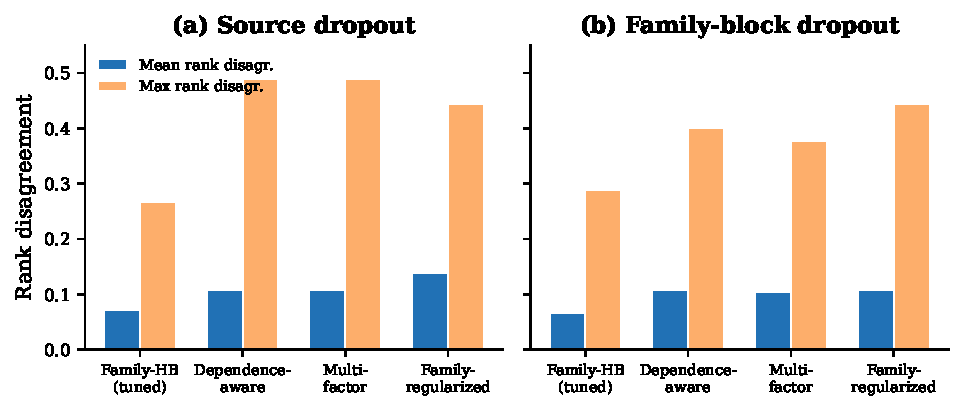
\includegraphics[width=\textwidth]{figures/fig1_robustness.pdf}
  \caption{Rank disagreement under source dropout and family-block dropout for four latent-truth model variants.
  Lower values indicate more stable rankings when evidence sources are removed.
  The tuned Family-HB model achieves the lowest disagreement under both protocols.}
  \label{fig:robustness}
\end{figure}

\begin{table}[t]
  \centering
  \caption{Robustness comparison across model variants.
  Family-HB (tuned) achieves the lowest mean and max rank disagreement under both stress protocols, as well as the smallest posterior prevalence shifts.}
  \label{tab:robustness}
  \small
  \begin{tabular}{@{}llccccc@{}}
    \toprule
    Protocol & Model & Mean rank & Max rank & Mean $|\Delta\pi|$ & Max $|\Delta\pi|$ & Mean $|\Delta\rho|$ \\
    \midrule
    \multirow{4}{*}{Source dropout}
      & \textbf{Family-HB (tuned)} & \textbf{0.072} & \textbf{0.267} & \textbf{0.015} & \textbf{0.062} & \textbf{0.001} \\
      & Dependence-aware           & 0.108 & 0.489 & 0.031 & 0.178 & 0.001 \\
      & Multifactor                & 0.108 & 0.489 & 0.036 & 0.191 & 0.004 \\
      & Family-regularized         & 0.139 & 0.444 & 0.041 & 0.102 & 0.023 \\
    \midrule
    \multirow{4}{*}{Family-block}
      & \textbf{Family-HB (tuned)} & \textbf{0.067} & \textbf{0.289} & \textbf{0.011} & \textbf{0.043} & \textbf{0.001} \\
      & Multifactor                & 0.104 & 0.378 & 0.017 & 0.069 & 0.005 \\
      & Family-regularized         & 0.107 & 0.444 & 0.037 & 0.075 & 0.022 \\
      & Dependence-aware           & 0.107 & 0.400 & 0.013 & 0.061 & 0.001 \\
    \bottomrule
  \end{tabular}
\end{table}

\subsection{The Context ``Uplift'' Is Almost Entirely a Base-Rate Effect}\label{sec:res-calibration}

\Cref{fig:calibration} shows that raw perturbation-calibration metrics are much higher in the context-matched universe: under matched Family-HB hyperparameters, precision@5000 is 0.043 versus 0.0014 in the full universe (a $30.7\times$ ratio), best F1 is 0.096 versus 0.004 ($26.0\times$), and best precision is 0.053 versus 0.002 ($23.2\times$).
\rev{Taken at face value these ratios suggest an order-of-magnitude ``calibration uplift'' from context matching. However, the two universes differ sharply in the density of \emph{evaluable} perturbation references: the context universe contains 237 reference edges among 7{,}536 candidates (base rate $3.14\%$), whereas the full universe contains 514 among 421{,}521 (base rate $0.122\%$). The base-rate ratio alone is $25.8\times$. Because precision scales with the base rate, most of the apparent uplift is a denominator artifact rather than superior ranking.}

\rev{To separate the two contributions we decompose the raw precision ratio multiplicatively into a base-rate term and a denominator-invariant \emph{signal} term (\Cref{eq:enrichment}):
\[
  \underbrace{\frac{\mathrm{P}@k_{\mathrm{ctx}}}{\mathrm{P}@k_{\mathrm{full}}}}_{\text{raw ratio}}
  \;=\;
  \underbrace{\frac{\text{base}_{\mathrm{ctx}}}{\text{base}_{\mathrm{full}}}}_{25.8\times}
  \times
  \underbrace{\frac{\mathrm{Enr}@k_{\mathrm{ctx}}}{\mathrm{Enr}@k_{\mathrm{full}}}}_{\approx1.4\times\ (k=5000)}.
\]
At the operating depth $k=5000$, the enrichment-over-random is $1.37\times$ in the context universe and $0.98\times$ (indistinguishable from random) in the full universe, so the genuine ranking difference between contexts is only $\approx1.4\times$ (\Cref{tab:calibration}, \Cref{fig:univ}). In other words, essentially all of the headline $23$--$31\times$ is attributable to the $25.8\times$ base-rate difference. This is the same denominator mechanism that inflates restricted-candidate metrics relative to universe-aware evaluation~\citep{kendiukhov2025universe}; the practical implication is not that context matching ``improves'' the model, but that raw precision is not comparable across universes and denominator-invariant enrichment (\Cref{eq:enrichment}) must be used instead.}

\rev{\Cref{fig:univ}a further shows that the denominator-invariant signal is weak and concentrated in coarse posterior-tie blocks: in the full universe the enrichment stays near or below $1\times$ across most of the ranking and rises only where a large block of tied high-posterior edges (heavily supported by curated references) enters, while in the context universe it peaks near $1.7\times$. The signal-to-noise ratio therefore does not improve smoothly with depth; it is dominated by a small number of high-consensus edges. This is precisely why the governance layer below relies on cross-universe consistency and enrichment rather than on either universe's raw precision.}

\begin{figure}[t]
  \centering
  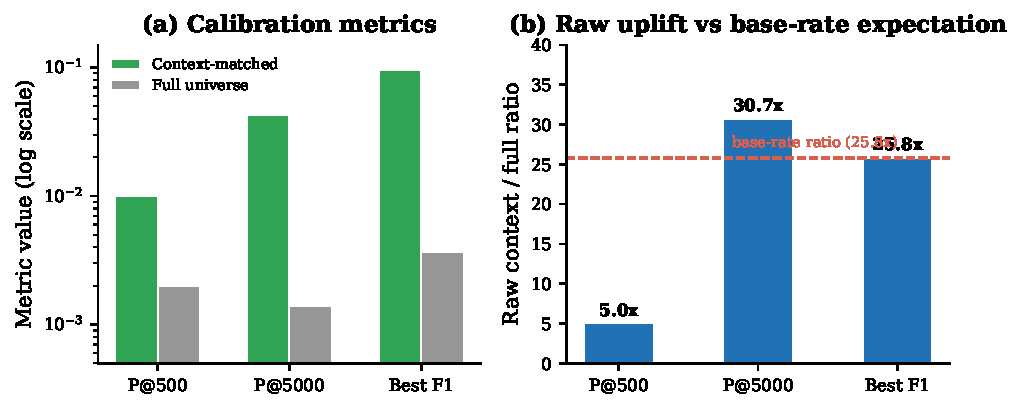
\includegraphics[width=\textwidth]{figures/fig2_calibration.pdf}
  \caption{(a) Raw calibration metrics in context-matched versus full-universe evaluation on a log scale.
  (b) The \rev{raw} ratio of context-matched to full-universe performance \rev{(23--31$\times$); as shown in \Cref{tab:calibration} and \Cref{fig:univ}, this ratio is dominated by the $25.8\times$ difference in reference base rate rather than by genuine ranking signal}.}
  \label{fig:calibration}
\end{figure}

\begin{table}[t]
  \centering
  \caption{\rev{Calibration metrics under matched Family-HB hyperparameters, decomposed into base-rate and denominator-invariant signal components. Raw precision is far higher in the context universe, but so is the reference base rate; the enrichment over random ($\mathrm{Enr}@k=\mathrm{P}@k/\text{base}$, \Cref{eq:enrichment}) shows the genuine ranking signal is modest in both. The raw P@5000 ratio ($30.7\times$) factors as base-rate ratio ($25.8\times$) $\times$ signal ratio ($1.4\times$).}}
  \label{tab:calibration}
  \small
  \begin{tabular}{@{}lccccc@{}}
    \toprule
    Universe & Ref.\ edges & Base rate & P@5000 & \rev{$\mathrm{Enr}@5000$} & Best F1 \\
    \midrule
    Context-matched & 237 & \rev{0.0314} & 0.043 & \rev{1.37$\times$} & 0.096 \\
    Full universe   & 514 & \rev{0.00122} & 0.0014 & \rev{0.98$\times$} & 0.004 \\
    \midrule
    \multicolumn{2}{@{}l}{\rev{Context / full ratio}} & \rev{25.8$\times$} & \rev{30.7$\times$} & \rev{1.4$\times$} & \rev{26.0$\times$} \\
    \bottomrule
  \end{tabular}
\end{table}

\rev{
\begin{figure}[t]
  \centering
  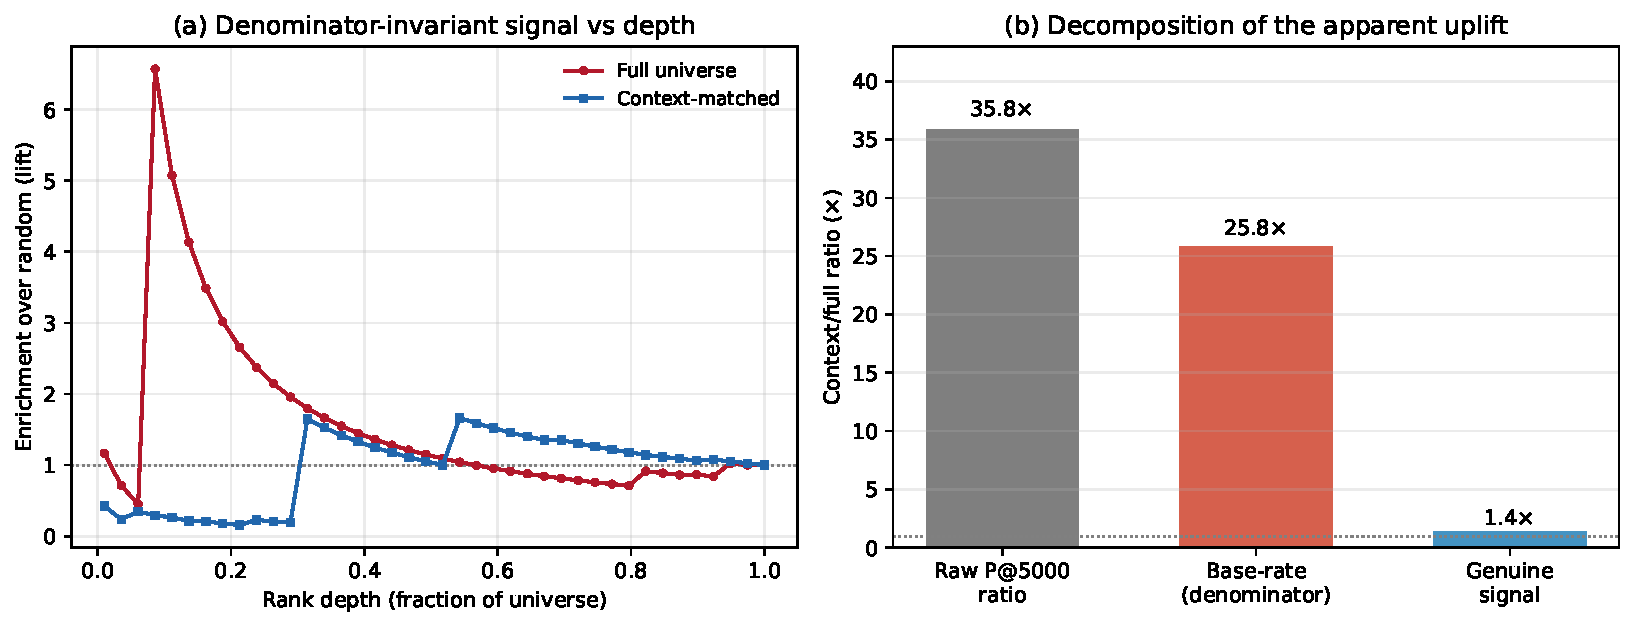
\includegraphics[width=\textwidth]{figures/fig7_universe_aware.pdf}
  \caption{Universe-aware view of the apparent calibration uplift.
  (a) Denominator-invariant enrichment over random as a function of rank depth in each universe: the genuine signal is weak (near or below $1\times$ over most of the ranking) and concentrated in coarse posterior-tie blocks.
  (b) Decomposition of the raw context/full precision@5000 ratio into a base-rate (denominator) factor of $25.8\times$ and a genuine-signal factor of $\approx1.4\times$.}
  \label{fig:univ}
\end{figure}
}

\subsection{Dual-Universe Governance Restricts Promotion to 0.2\% of Candidates}\label{sec:res-governance}

The dual-universe governance policy (\Cref{fig:governance}) assigns edges to four tiers: 500 Strong, 342 Moderate, 8,316 Conditional, and 412,363 Exploratory.
Only the 842 Strong and Moderate edges (0.2\% of the full universe, 11.2\% of context edges) are eligible for promotion as evidence-backed claims; the remaining 99.8\% are reported either as structured hypotheses (Conditional) or as exploratory leads.

Cross-universe tier consistency is limited: exact tier agreement is 5.6\% and within-one-tier agreement is 63.9\%, with a mean absolute tier gap of 1.31.
This substantial disagreement between evaluation contexts is precisely why dual-universe governance is necessary: edges that appear strong in one context may rank poorly in the other, and single-universe evaluation would miss this discrepancy.

\begin{figure}[t]
  \centering
  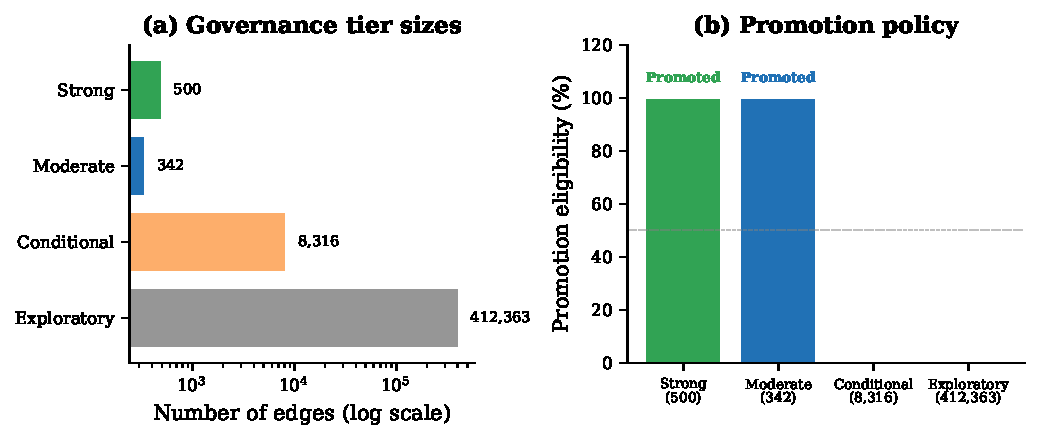
\includegraphics[width=\textwidth]{figures/fig3_governance.pdf}
  \caption{(a) Number of edges assigned to each governance tier (log scale).
  The vast majority of candidate edges fall in the Exploratory tier.
  (b) Perturbation enrichment by tier: Strong and Moderate edges exceed the 1.5$\times$ endpoint threshold, while Conditional and Exploratory edges fall near or below random expectation.}
  \label{fig:governance}
\end{figure}

\rev{
Because promotion merges the Strong (500 edges) and Moderate (342 edges) tiers, we report their validation profiles separately (\Cref{tab:strongmod}) so that downstream users can judge the risk/return of each. The Strong tier is both more diverse (58 unique TFs versus 21) and more strongly supported by the genuinely external ChIP-seq references (\Cref{sec:res-external}): its enrichment on the strict ENETS2 sequence-specific set is $2.12\times$ ($p=2.0\times10^{-8}$), whereas the Moderate tier reaches only $1.32\times$ ($p=0.075$, not significant) and is more concentrated (top-2 TF fraction $0.73$ versus $0.50$). On the permissive ENCODE TFBS set both tiers are comparable ($1.79\times$ versus $1.74\times$, both $p<10^{-40}$). The Moderate tier therefore extends coverage rather than diversity, and its inclusion should be viewed as a recall-oriented, lower-specificity extension of the promoted set.
}

\rev{
\begin{table}[t]
  \centering
  \caption{\rev{Distinct validation profile of the Strong and Moderate promoted tiers. External enrichments are computed against genuinely external ChIP-seq references (\Cref{sec:res-external}) on the ENCODE-evaluable candidate subspace.}}
  \label{tab:strongmod}
  \small
  \begin{tabular}{@{}lccccc@{}}
    \toprule
    Tier & Edges & Unique TFs & Top-2 TF frac. & ENCODE enr. & ENETS2 (strict) enr. \\
    \midrule
    Strong   & 500 & 58 & 0.50 & 1.79$\times$ ($p{<}10^{-62}$) & 2.12$\times$ ($p{=}2.0{\times}10^{-8}$) \\
    Moderate & 342 & 21 & 0.73 & 1.74$\times$ ($p{<}10^{-40}$) & 1.32$\times$ ($p{=}0.075$) \\
    \bottomrule
  \end{tabular}
\end{table}
}

\rev{
\paragraph{Cutoff sensitivity.}
The tier rank budgets $(k_1,k_2,k_3)=(500,5000,20000)$ are heuristic. Rescaling all three simultaneously by $\pm10\%$ leaves the promoted pool and its conclusions essentially unchanged: the promoted count moves only from 842 to 834 (at $\times0.9$) or 849 (at $\times1.1$), the top-1 and top-2 TF fractions shift by $<0.7$ percentage points, and the external ENCODE enrichment is invariant to three significant figures ($1.768\times$ at $\times1.0$ versus $1.768\times$ and $1.760\times$ at $\times0.9$ and $\times1.1$; all $p<10^{-102}$). The governance conclusions are therefore not artifacts of the exact cutoff values.
}

\subsection{Source Concentration Is High but Partially Controllable}\label{sec:res-concentration}

The promoted edge set, while small, exhibits high source concentration: the top transcription factor (EGR1) accounts for 32.2\% of promoted edges, and the top two TFs (EGR1, ETS1) account for 59.0\% (\Cref{fig:concentration}a).
By contrast, the Conditional tier is much more diverse (top-1 source fraction 4.3\%, 885 unique sources versus 60 in the promoted set).

A deconcentration policy sweep (\Cref{fig:concentration}b) shows that mild penalization ($\alpha = 0.05$) at an intermediate promotion budget (500 edges) reduces top-1 concentration from 26.6\% to 22.6\% without any loss in perturbation-backed reference precision.
However, the relationship between deconcentration and validation performance is budget-dependent: at a tight budget of 300 edges, deconcentration reduces concentration sharply (from 43.3\% to 15.0\%) but at the cost of losing perturbation-validated hits (4 to 1), while at higher budgets ($\geq$700) the baseline policy is already optimal (\Cref{tab:deconcentration}).

\begin{figure}[t]
  \centering
  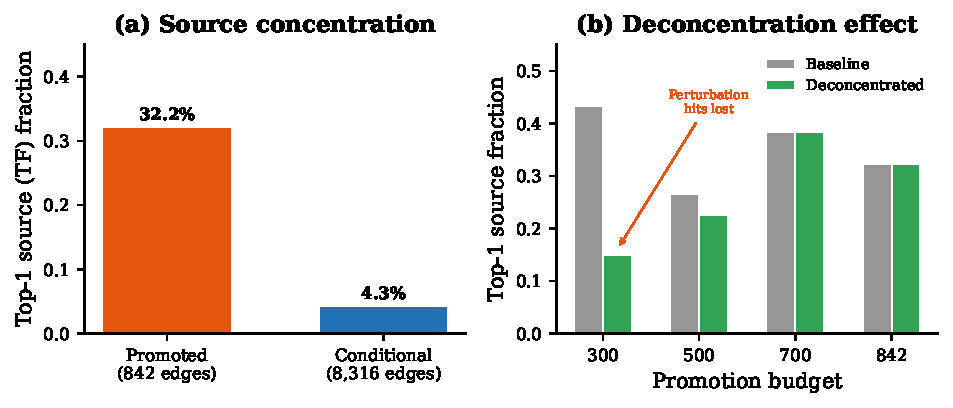
\includegraphics[width=\textwidth]{figures/fig4_concentration.pdf}
  \caption{(a) Top-1 TF source fraction in promoted versus conditional edge sets.
  (b) Deconcentration effect across promotion budgets: mild penalization reduces concentration at intermediate budgets without validation loss, but harms perturbation recovery at tight budgets.}
  \label{fig:concentration}
\end{figure}

\begin{table}[t]
  \centering
  \caption{Budget sensitivity of deconcentration governance.
  At budget 500, deconcentration reduces concentration without perturbation loss; at budget 300, it trades concentration for perturbation hits.}
  \label{tab:deconcentration}
  \small
  \begin{tabular}{@{}lcccc@{}}
    \toprule
    Budget & Policy & $\Delta$ top-1 frac. & $\Delta$ high-overlap hits & $\Delta$ ref.\ prec. \\
    \midrule
    300 & Penalized ($\alpha$=0.05) & $-$0.283 & $-$3 & $-$0.010 \\
    500 & Penalized ($\alpha$=0.05) & $-$0.040 &  0   &  0 \\
    700 & Baseline                  &  0       &  0   &  0 \\
    842 & Baseline                  &  0       &  0   &  0 \\
    \bottomrule
  \end{tabular}
\end{table}

\rev{
\paragraph{Automated operating-point selection.}
The budget-dependence above means no single hand-picked promotion budget is obviously correct. We therefore select the operating point automatically. Over a grid of promotion budgets and source penalties $(\text{budget},\alpha)$, we measure source diversity as the Pielou evenness $J=H/\ln n$ of the promoted-TF distribution ($H$ = Shannon entropy) and validation precision as the enrichment against the external ENCODE reference, then choose the point maximizing the harmonic mean of the two min--max-normalized criteria (a diversity--precision $F$-score; the knee of the frontier gives an identical choice). The selected point is a budget of 200 edges at $\alpha=0.05$ (\Cref{fig:frontier}): it cuts the top-1 TF fraction from $0.32$ to $0.06$ and raises evenness from $0.31$ to $0.70$ while \emph{preserving} external enrichment ($1.79\times$, $p=1.5\times10^{-20}$, versus $1.77\times$ at the fixed 842-edge budget). Crucially, the external enrichment is essentially flat ($1.6$--$1.8\times$) across the entire grid: against a dense external reference, deconcentration carries no precision penalty. The apparent penalty in \Cref{tab:deconcentration} is specific to the sparse perturbation panels, where the promoted set intersects only a handful of reference edges and the hit count is dominated by sampling noise.

\paragraph{Functional characterization.}
Enrichment analysis of the promoted target genes~\citep{kuleshov2016enrichr} (\Cref{tab:function}) shows that the promoted set is dominated by generic transcriptional-regulation terms and by mitogen/stress and cell-cycle hub programs (TNF-$\alpha$/NF-$\kappa$B signaling, E2F targets, G2--M checkpoint, mTORC1; KEGG cell cycle and cellular senescence). This confirms that dual-universe governance preferentially promotes densely annotated master-regulator hubs, a direct consequence of curation bias in the reference databases. However, the framework is not \emph{structurally} confined to housekeeping hubs: removing the three dominant hubs (EGR1, ETS1, E2F4) and re-running enrichment on the residual ``peripheral'' targets surfaces context-appropriate immune programs for these immune-tissue cohorts---interferon-$\gamma$ response, cytokine-mediated signaling, and allograft rejection (all adjusted $p<10^{-3}$)---indicating that peripheral promoted edges do carry cell-type-relevant signal, albeit at lower confidence than the hubs.

\begin{table}[t]
  \centering
  \caption{\rev{Top functional enrichment (Enrichr; adjusted $p$) of promoted target genes, for the full promoted set and for the ``peripheral'' set obtained after removing the three dominant hub TFs. The full set is hub/stress-dominated; the peripheral set surfaces immune-context-specific programs.}}
  \label{tab:function}
  \small
  \begin{tabular}{@{}llc@{}}
    \toprule
    Gene set & Representative enriched program & Adj.\ $p$ \\
    \midrule
    Promoted (all, 600 genes)   & TNF-$\alpha$ signaling via NF-$\kappa$B (Hallmark) & $3.9\times10^{-20}$ \\
                                & E2F targets (Hallmark)                             & $1.7\times10^{-19}$ \\
                                & Cell cycle (KEGG)                                  & $7.5\times10^{-11}$ \\
    \midrule
    Peripheral (89 genes)       & Interferon-$\gamma$ response (Hallmark)            & $2.4\times10^{-7}$ \\
                                & Cytokine-mediated signaling (GO:BP)                & $1.6\times10^{-4}$ \\
                                & Allograft rejection (Hallmark)                     & $1.8\times10^{-4}$ \\
    \bottomrule
  \end{tabular}
\end{table}

\begin{figure}[t]
  \centering
  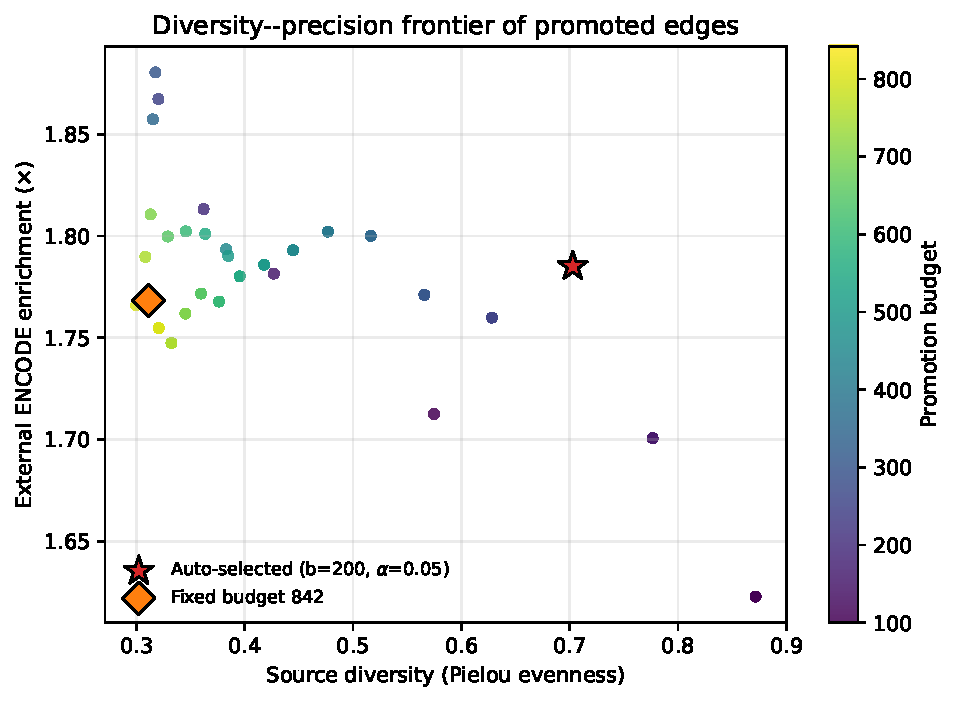
\includegraphics[width=0.72\textwidth]{figures/fig8_deconcentration_frontier.pdf}
  \caption{\rev{Diversity--precision frontier of promoted edges over the $(\text{budget},\alpha)$ grid. Each point is an operating policy, colored by budget; the $y$-axis is enrichment against the external ENCODE reference and the $x$-axis is source evenness. External precision is nearly flat across the grid, so the automatically selected point (star: budget 200, $\alpha=0.05$) achieves far higher diversity than the fixed 842-edge budget (diamond) at no precision cost.}}
  \label{fig:frontier}
\end{figure}
}

\subsection{External Validation Against Perturbation and ChIP-seq References}\label{sec:res-external}

Under a manifest-locked external protocol that freezes all policy-search parameters before evaluation, the promoted edge set at budget 4,000 achieves enrichment of $2.21\times$ over candidate-space random expectation ($p = 4.15 \times 10^{-86}$) on reserved perturbation panels.
This enrichment is a denominator-invariant lift over random (\Cref{eq:enrichment}) and is therefore not subject to the base-rate confound of \Cref{sec:res-calibration}.
Structural score calibration raises full-universe metrics to precision@5000 = 0.037 and best F1 = 0.117, confirming that the framework's conservative governance does not sacrifice detectable biological signal.

\rev{
\paragraph{A genuinely external ChIP-seq reference.}
All references used inside the credibility model are curated interaction or perturbation resources. To test the promoted set against evidence of an entirely different modality that never enters the fusion, we use the ENCODE TFBS ChIP-seq clustered network (5-cell-line union; 184 assayed TFs, $1.5\times10^6$ TF--target edges)~\citep{encode2012integrated} and, as a stricter companion, the ENCODE ENETS2 sequence-specific network (90 TFs). Neither is a source, family, or panel anywhere in the pipeline. We restrict the candidate space to edges whose TF is assayed in the external set (universe-aware: 16{,}852 edges for ENCODE, base rate $47.4\%$; 16{,}239 for ENETS2, base rate $6.6\%$) and compute the enrichment of each governance tier over that base rate, with hypergeometric significance.

The results (\Cref{tab:external}) show a clean, monotone separation across tiers on both references. The promoted (Strong$+$Moderate) pool is enriched $1.77\times$ on ENCODE ($658/785$ edges confirmed; $p=2.3\times10^{-104}$) and $1.77\times$ on the strict ENETS2 set ($p=6.2\times10^{-8}$); the Strong tier reaches $2.12\times$ on the strict set. Enrichment declines monotonically to the Conditional tier ($1.17\times$/$1.04\times$) and falls below random for the Exploratory tier ($0.89\times$/$0.93\times$), exactly as the governance ordering predicts. This external, cross-modality agreement is the strongest single piece of evidence that the promoted set reflects genuine regulatory structure rather than curation artifacts of the internal references.

\begin{table}[t]
  \centering
  \caption{\rev{Enrichment of governance tiers against two genuinely external ChIP-seq references never used in the credibility model, over the ENCODE-evaluable candidate subspace. Enrichment is the tier precision divided by the candidate-space base rate; $p$ is the hypergeometric upper-tail probability.}}
  \label{tab:external}
  \small
  \begin{tabular}{@{}lcccc@{}}
    \toprule
     & \multicolumn{2}{c}{ENCODE TFBS (permissive)} & \multicolumn{2}{c}{ENETS2 seq-specific (strict)} \\
    \cmidrule(lr){2-3}\cmidrule(lr){4-5}
    Tier & Enrichment & $p$ & Enrichment & $p$ \\
    \midrule
    Strong                    & 1.79$\times$ & $5\times10^{-63}$  & 2.12$\times$ & $2.0\times10^{-8}$ \\
    Moderate                  & 1.74$\times$ & $4\times10^{-41}$  & 1.32$\times$ & $0.075$ \\
    \textbf{Promoted (S+M)}   & \textbf{1.77$\times$} & $\mathbf{2\times10^{-104}}$ & \textbf{1.77$\times$} & $\mathbf{6\times10^{-8}}$ \\
    Conditional               & 1.17$\times$ & $1\times10^{-32}$  & 1.04$\times$ & $0.22$ \\
    Exploratory               & 0.89$\times$ & $1.00$             & 0.93$\times$ & $1.00$ \\
    \bottomrule
  \end{tabular}
\end{table}
}

\subsection{Leave-One-Cohort-Out Replication: 5/6 Pass with Support-Stratified Reliability}\label{sec:res-replication}

Leave-one-cohort-out replication across six perturbation cohorts (\Cref{fig:replication}a) yields five passes and one failure (pass rate 0.833; Wilson 95\% CI [0.436, 0.970]).
The five passing cohorts show enrichments in the range 2.16--2.29 with strong significance ($p \ll 0.05$), while the failing cohort (Shifrut, CRISPR-KO in T cells) shows enrichment of only 0.33 with $p = 0.98$ and has only 7 external candidate-space reference edges.

Support-stratified analysis (\Cref{fig:replication}b) reveals a clear reliability threshold: all cohorts with $\geq$10 external reference edges pass the endpoint criterion (4/4), while cohorts with fewer than 10 edges show a 50\% pass rate (1/2).
This provides an operational reliability floor: cohorts below the support threshold should be classified as underpowered rather than definitively negative.

\begin{figure}[t]
  \centering
  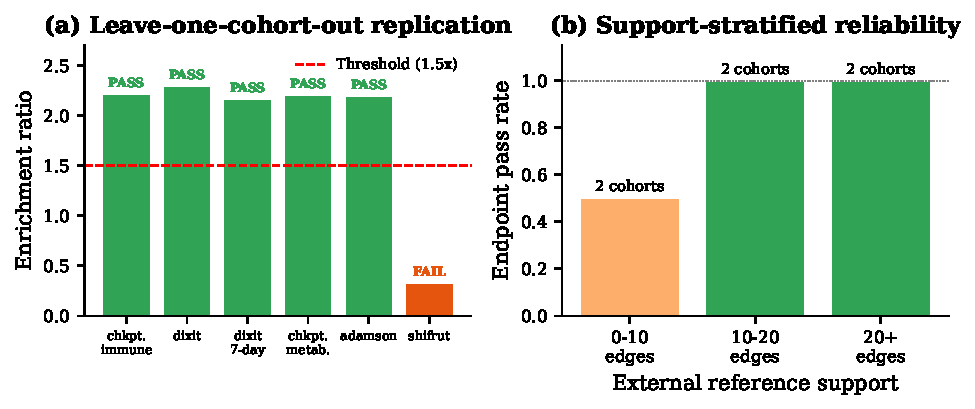
\includegraphics[width=\textwidth]{figures/fig5_replication.pdf}
  \caption{(a) Leave-one-cohort-out enrichment across six perturbation cohorts.
  The dashed line indicates the $1.5\times$ enrichment threshold.
  Five cohorts pass; the Shifrut cohort fails due to sparse reference support.
  (b) Support-stratified reliability: cohorts with $\geq$10 reference edges achieve 100\% pass rate.}
  \label{fig:replication}
\end{figure}

\subsection{Cohort-Omission Fragility Is Localized}\label{sec:res-fragility}

Bayesian endpoint modeling with covariate-aware MCMC hierarchical priors provides continuous confidence estimates.
Support-eligible cohorts ($\geq$10 reference edges) achieve mean posterior pass probability of 0.96, while support-limited cohorts average 0.23.
Multilevel prior-sensitivity analysis across five hyperprior profiles confirms that tier assignments are stable for all cohorts (one distinct tier per cohort across all profiles), indicating that the remaining uncertainty is data-support-limited rather than prior-specification-limited.

Leave-one-cohort-out, leave-two-cohort-out, and leave-three-cohort-out stress protocols (\Cref{fig:fragility}) show that endpoint probability drift increases modestly with stress severity (mean $|\Delta p|$: 0.025 $\rightarrow$ 0.043 $\rightarrow$ 0.049), but tier instability remains localized to a single cohort (Shifrut, 1/6) across all three levels.
Even when half of all cohorts are removed per run (L3O), high-support cohort tiers remain stable, confirming that the framework's conclusions are robust to cohort-composition perturbations.

\begin{figure}[t]
  \centering
  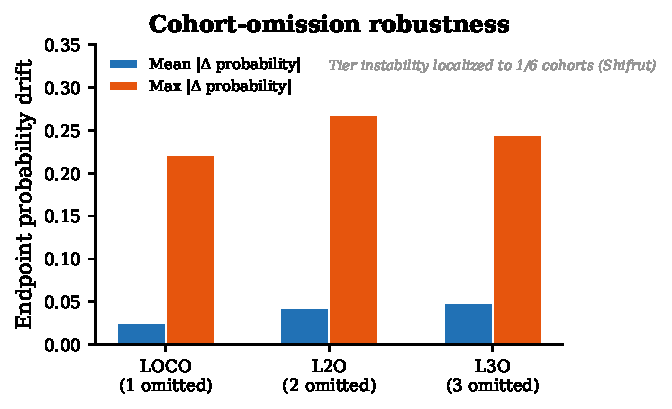
\includegraphics[width=0.65\textwidth]{figures/fig6_fragility.pdf}
  \caption{Endpoint probability drift under increasing cohort-omission stress.
  Mean drift increases modestly from LOCO to L3O, but tier instability remains confined to 1/6 cohorts.}
  \label{fig:fragility}
\end{figure}

% ======================================================================
% 6. DISCUSSION
% ======================================================================
\section{Discussion}\label{sec:discussion}

The central finding of this work is that the standard single-reference evaluation paradigm for GRN benchmarking systematically misrepresents the reliability of predicted regulatory edges, and that a multi-reference latent truth framework can provide substantially more calibrated and honest assessments of predictive quality.

\rev{The most important methodological lesson concerns how \emph{not} to read the $23$--$31\times$ gap between the context-matched and full universes. That gap is real for raw precision, but our decomposition (\Cref{sec:res-calibration}) shows it is almost entirely a base-rate artifact: the context universe simply has a $25.8\times$ higher density of evaluable references, and once metrics are normalized to a denominator-invariant enrichment the genuine ranking difference between contexts is only $\approx1.4\times$. Reporting the raw ratio as a ``calibration uplift'' would therefore overstate what context matching buys, in the same way that restricting the candidate set inflates precision metrics without improving the underlying predictions~\citep{kendiukhov2025universe}. The constructive takeaway is not that context matching makes the model better, but that cross-universe precision comparisons are not meaningful and that promotion and validation must rest on denominator-invariant enrichment---which is what the governance layer does, and why the promoted set nonetheless shows a genuine $\approx1.8$--$2.2\times$ enrichment against both held-out perturbation panels and an external ChIP-seq reference.}

The dual-universe governance framework addresses a different problem: how to translate continuous credibility scores into discrete, defensible claims about which predicted regulatory edges are trustworthy enough to report.
The extreme conservatism of the framework (promoting only 0.2\% of candidates) is intentional.
In a field where benchmark inflation and overconfident claims are persistent concerns~\citep{pratapa2020benchmarking}, we argue that explicit governance policies with traceable promotion criteria are preferable to arbitrary score thresholds, even if they result in smaller claim sets.

The source concentration issue (top-2 TFs accounting for $\sim$59\% of promoted edges) reflects a genuine property of the underlying data rather than a methodological artifact: some TFs have much denser reference coverage and therefore accumulate more evidence, and the functional analysis confirms that the promoted set is dominated by densely annotated master-regulator hub and stress programs.
\rev{Two findings temper this. First, an automated diversity--precision criterion (\Cref{sec:res-concentration}) removes the need for a hand-picked budget and recovers a far more even promoted set (top-1 TF fraction $0.32\rightarrow0.06$) at no cost in external-reference precision, because enrichment against a dense external reference is essentially flat across the operating grid. Second, the residual peripheral edges do carry cell-type-appropriate signal (interferon-$\gamma$, cytokine, and allograft-rejection programs for these immune cohorts). We nonetheless state the corresponding limitation plainly: the framework cannot \emph{confirm} weakened, context-specific peripheral pathways using the sparse perturbation panels, where forcing diversity collapses the already tiny validated-hit counts (\Cref{tab:deconcentration}); such peripheral promotions should be treated as lower-confidence hypotheses that require denser or bespoke perturbation validation.}

The LOCO replication results provide both reassurance and a concrete limitation.
The 5/6 pass rate with strong enrichment in passing cohorts suggests that the framework captures genuine biological signal.
The single failure, cleanly attributable to sparse reference support rather than model collapse, suggests a practical reliability criterion: users should verify that their evaluation context has sufficient perturbation reference coverage before interpreting negative results as evidence against model quality.
\rev{We deliberately state this as an exploratory rather than an established threshold. With only six cohorts---four above and two below the ten-edge support line---the pass rate carries a wide Wilson interval ([0.44, 0.97]), the support cutoff is estimated from a handful of points, and the cohort-level Bayesian model can support only minimal covariate structure. The support-density criterion should therefore be read as a hypothesis to be re-estimated on a larger cohort panel, not as a calibrated operating boundary.}

\paragraph{Limitations.}
Five limitations constrain the current work.
First, all analyses are conducted on scGPT embeddings from immune tissue cohorts; generalization to other models (e.g., Geneformer) and other tissue contexts remains to be tested.
Second, perturbation overlap in the full universe is sparse (514 out of 421,521 edges), limiting direct perturbation-validation power; \rev{this sparsity is also why we add a dense external ChIP-seq anchor (\Cref{sec:res-external}) and why small-budget perturbation precision estimates are noisy.}
Third, the dual-governance thresholds are rule-based rather than learned; \rev{we now report their exact values and a $\pm10\%$ sensitivity analysis (\Cref{sec:res-governance}), but the ordinal alignment procedure should still be validated prospectively on independent cohorts.}
Fourth, cohort-level Bayesian modeling operates on only six cohorts, supporting limited covariate structure, \rev{so all cohort-level conclusions---including the support-density reliability threshold---are exploratory and require a larger cohort panel for confirmation.}
\rev{Fifth, the references used \emph{inside} the credibility model are curated interaction and perturbation resources; we mitigate the resulting circularity by validating the promoted set against an external ChIP-seq reference (ENCODE) that is not part of the fusion, but replication against additional independently curated references in non-immune contexts would strengthen the claims further.}

% ======================================================================
% 7. CONCLUSION
% ======================================================================
\section{Conclusion}\label{sec:conclusion}

We have presented a multi-reference latent truth framework for GRN benchmarking that replaces the single-reference evaluation paradigm with explicit probabilistic credibility modeling under source dependence.
The hierarchical Family-Bayes estimator achieves the highest robustness under structured stress tests, \rev{a universe-aware decomposition shows that the large apparent gap between full- and context-universe precision is a base-rate artifact and that denominator-invariant enrichment is the correct cross-universe quantity}, and a four-tier dual-universe governance policy provides traceable, conservative claim promotion.
\rev{Pre-registered replication across six perturbation cohorts, together with validation against a genuinely external ChIP-seq reference, indicates that the promoted set captures genuine biological signal ($\approx1.8$--$2.2\times$ enrichment), while the small cohort count means the support-dependent reliability boundary should be treated as exploratory.}

The framework is lightweight (all analyses run on a laptop without GPU), reproducible (all artifacts are checksum-manifested), and intentionally conservative, prioritizing calibrated uncertainty over inflated claims.
We hope it contributes to more honest and context-aware evaluation practices in the rapidly growing field of mechanistic interpretability for single-cell foundation models.

% ======================================================================
% DATA AND CODE AVAILABILITY
% ======================================================================
\section*{Data and Code Availability}

All source code, analysis pipelines, and summary data tables required to reproduce the results and figures in this paper are publicly available at \url{https://github.com/Biodyn-AI/multireference-latent-truth}.
The repository includes model fitting scripts, robustness stress protocols, governance enforcement, replication analyses, and figure generation code.
All model fitting is CPU-only and requires only standard scientific Python packages (numpy, scipy, pandas, matplotlib).

% ======================================================================
% ACKNOWLEDGMENTS
% ======================================================================
\section*{Acknowledgments}

The author thanks the open-source communities behind scGPT, DoRothEA, TRRUST, ENCODE, Enrichr, and the Perturb-seq datasets that made this analysis possible.

% ======================================================================
% REFERENCES
% ======================================================================
\begin{thebibliography}{25}

\bibitem[Adamson et~al.(2016)]{adamson2016multiplexed}
Adamson, B., Norman, T.~M., Jost, M., et~al.
\newblock A multiplexed single-cell {CRISPR} screening platform enables systematic dissection of the unfolded protein response.
\newblock \emph{Cell}, 167(7):1867--1882, 2016.

\bibitem[Aibar et~al.(2017)]{aibar2017scenic}
Aibar, S., Gonz{\'a}lez-Blas, C.~B., Moerman, T., et~al.
\newblock {SCENIC}: Single-cell regulatory network inference and clustering.
\newblock \emph{Nature Methods}, 14(11):1083--1086, 2017.

\bibitem[Bravo Gonz{\'a}lez-Blas et~al.(2023)]{bravo2023scenic}
Bravo Gonz{\'a}lez-Blas, C., De~Winter, S., Hulselmans, G., et~al.
\newblock {SCENIC+}: Single-cell multiomic inference of enhancers and gene regulatory networks.
\newblock \emph{Nature Methods}, 20(9):1355--1367, 2023.

\bibitem[Cui et~al.(2024)]{cui2024scgpt}
Cui, H., Wang, C., Maan, H., et~al.
\newblock sc{GPT}: Towards building a foundation model for single-cell multi-omics using generative {AI}.
\newblock \emph{Nature Methods}, 2024.

\bibitem[Dawid and Skene(1979)]{dawid1979maximum}
Dawid, A.~P. and Skene, A.~M.
\newblock Maximum likelihood estimation of observer error-rates using the {EM} algorithm.
\newblock \emph{Journal of the Royal Statistical Society: Series C}, 28(1):20--28, 1979.

\bibitem[ENCODE Project Consortium(2012)]{encode2012integrated}
The {ENCODE} Project Consortium.
\newblock An integrated encyclopedia of {DNA} elements in the human genome.
\newblock \emph{Nature}, 489(7414):57--74, 2012.

\bibitem[Dixit et~al.(2016)]{dixit2016perturb}
Dixit, A., Parnas, O., Li, B., et~al.
\newblock Perturb-seq: Dissecting molecular circuits with scalable single-cell {RNA} profiling of pooled genetic screens.
\newblock \emph{Cell}, 167(7):1853--1866, 2016.

\bibitem[Garc{\'i}a-Alonso et~al.(2019)]{garcia2019benchmark}
Garc{\'i}a-Alonso, L., Holland, C.~H., Ibrahim, M.~M., Turei, D., and Saez-Rodriguez, J.
\newblock Benchmark and integration of resources for the estimation of human transcription factor activities.
\newblock \emph{Genome Research}, 29(8):1363--1375, 2019.

\bibitem[Han et~al.(2018)]{han2018trrust}
Han, H., Cho, J.-W., Lee, S., et~al.
\newblock {TRRUST} v2: An expanded reference database of human and mouse transcriptional regulatory interactions.
\newblock \emph{Nucleic Acids Research}, 46(D1):D199--D202, 2018.

\bibitem[Hao et~al.(2024)]{hao2024large}
Hao, M., Gong, J., Yuan, Y., et~al.
\newblock Large-scale foundation model on single-cell transcriptomics.
\newblock \emph{Nature Methods}, 2024.

\bibitem[Huynh-Thu et~al.(2010)]{huynh2010inferring}
Huynh-Thu, V.~A., Irrthum, A., Wehenkel, L., and Geurts, P.
\newblock Inferring regulatory networks from expression data using tree-based methods.
\newblock \emph{PLOS ONE}, 5(9):e12776, 2010.

\bibitem[Jackson et~al.(2020)]{jackson2020gene}
Jackson, C.~A., Castro, D.~M., Saldi, G.-A., Bonneau, R., and Bhatt, D.
\newblock Gene regulatory network reconstruction using single-cell {RNA} sequencing of barcoded genotypes in diverse environments.
\newblock \emph{eLife}, 9:e51254, 2020.

\bibitem[Kamimoto et~al.(2023)]{kamimoto2023dissecting}
Kamimoto, K., Hoffmann, C.~M., and Morris, S.~A.
\newblock {CellOracle}: Dissecting cell identity via network inference and \emph{in silico} gene perturbation.
\newblock \emph{Nature}, 614:742--751, 2023.

\bibitem[Kendiukhov(2026)]{kendiukhov2025universe}
Kendiukhov, I.
\newblock Evaluation protocol choices dominate reported performance in gene regulatory network benchmarks for single-cell foundation models.
\newblock \emph{Research Square preprint}, 2026.
\newblock doi:10.21203/rs.3.rs-9283852/v1.

\bibitem[Moerman et~al.(2019)]{moerman2019grnboost2}
Moerman, T., Santos, S.~A., Gonz{\'a}lez-Blas, C.~B., et~al.
\newblock {GRNBoost2} and {Arboreto}: Efficient and scalable inference of gene regulatory networks.
\newblock \emph{Bioinformatics}, 35(12):2159--2161, 2019.

\bibitem[Kuleshov et~al.(2016)]{kuleshov2016enrichr}
Kuleshov, M.~V., Jones, M.~R., Rouillard, A.~D., et~al.
\newblock {Enrichr}: A comprehensive gene set enrichment analysis web server 2016 update.
\newblock \emph{Nucleic Acids Research}, 44(W1):W90--W97, 2016.

\bibitem[Pratapa et~al.(2020)]{pratapa2020benchmarking}
Pratapa, A., Jalihal, A.~P., Law, J.~N., Bharadwaj, A., and Murali, T.~M.
\newblock Benchmarking algorithms for gene regulatory network inference from single-cell transcriptomic data.
\newblock \emph{Nature Methods}, 17(2):147--154, 2020.

\bibitem[Raykar et~al.(2010)]{raykar2010learning}
Raykar, V.~C., Yu, S., Zhao, L.~H., et~al.
\newblock Learning from crowds.
\newblock \emph{Journal of Machine Learning Research}, 11:1297--1322, 2010.

\bibitem[Replogle et~al.(2022)]{replogle2022mapping}
Replogle, J.~M., Saunders, R.~A., Pogson, A.~N., et~al.
\newblock Mapping information-rich genotype-phenotype landscapes with genome-scale {Perturb-seq}.
\newblock \emph{Cell}, 185(14):2559--2575, 2022.

\bibitem[Schiebinger et~al.(2019)]{schiebinger2019optimal}
Schiebinger, G., Shu, J., Tabaka, M., et~al.
\newblock Optimal-transport analysis of single-cell gene expression identifies developmental trajectories in reprogramming.
\newblock \emph{Cell}, 176(4):928--943, 2019.

\bibitem[Theodoris et~al.(2023)]{theodoris2023transfer}
Theodoris, C.~V., Xiao, L., Chopra, A., et~al.
\newblock Transfer learning enables predictions in network biology.
\newblock \emph{Nature}, 618:616--624, 2023.

\bibitem[Tseng et~al.(2012)]{tseng2012comprehensive}
Tseng, G.~C., Ghosh, D., and Feingold, E.
\newblock Comprehensive literature review and statistical considerations for microarray meta-analysis.
\newblock \emph{Nucleic Acids Research}, 40(9):3785--3799, 2012.

\bibitem[Zheng et~al.(2017)]{zheng2017massively}
Zheng, G.~X.~Y., Terry, J.~M., Belgrader, P., et~al.
\newblock Massively parallel digital transcriptional profiling of single cells.
\newblock \emph{Nature Communications}, 8:14049, 2017.

\end{thebibliography}

\end{document}
